\chapter[Introdução]{Introdução}

A crescente demanda energética e a preocupação com os impactos ambientais advindos do uso de combustíveis fósseis como fonte de energia têm levado ao incentivo da inserção de fontes alternativas que sejam limpas e renováveis na matriz energética nacional de países em todo o mundo. O Brasil se destaca no cenário mundial por ter uma oferta interna de energia elétrica com ampla participação de fontes renováveis, as quais foram responsáveis por 81,7\% da energia elétrica ofertada no ano de 2016 \cite{mme2017}. Na Figura \ref{figura_matriz}, é possível visualizar o gráfico da Oferta Interna de Energia Elétrica por fonte para o ano de 2016, segundo dados do Ministério de Minas e Energia (MME).

\begin{figure}[!htb]
	\centering
	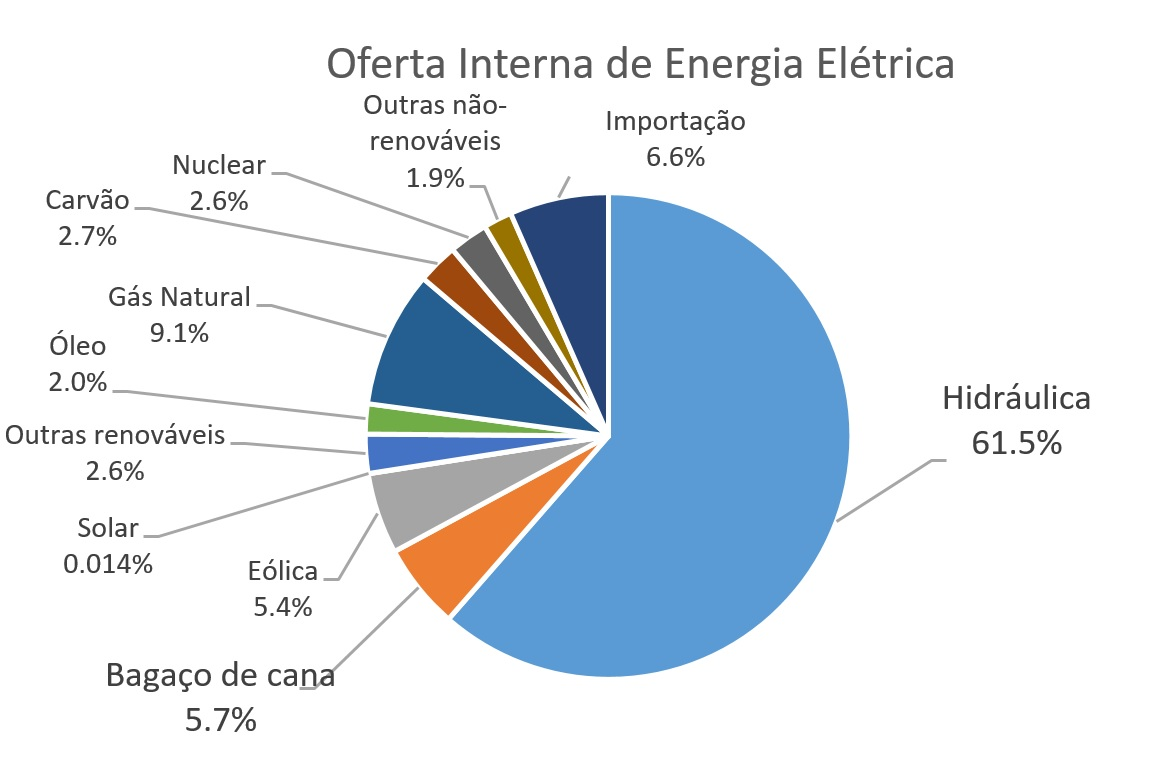
\includegraphics{OIEE}
	\caption{Oferta Interna de Energia Elétrica por fonte \cite{mme2017}}
	\label{figura_matriz}
\end{figure}

Do total da oferta, 61,5\% são provenientes da energia hídrica, o que torna a matriz energética nacional predominantemente limpa. O percentual das demais fontes renováveis somam 16,3\%, ultrapassando o somatório das não renováveis que totalizam 15,6\%. A energia solar, apesar de ter crescido em relação ao ano anterior, ainda apresenta baixa representatividade, a energia eólica, por outro lado, além do crescimento, apresenta significativa participação na matriz.

Dentre as biomassas, o bagaço da cana de açúcar é o principal responsável pela oferta de energia elétrica nacional, com um percentual de 5,7\%. Sua principal aplicação acontece nas usinas sucroalcooleiras, que o usam em processos de cogeração de energia para a autossuficiência em energias térmica e elétrica, vendendo o excedente deste último para a rede do sistema elétrico nacional. Para esse processo de cogeração, o bagaço resultante da moagem da cana para a obtenção de açúcar e álcool é queimado em uma caldeira e o calor resultante irá aquecer um fluido, geralmente água, gerando vapor que movimentará uma turbina acoplada a um gerador de energia elétrica. Outra forma de obtenção de energia elétrica através da biomassa se dá pelo processo de gaseificação, o qual transforma o combustível sólido em um gás de síntese, que movimentará um motor ou uma turbina acoplados a um gerador. A gaseificação apresenta vantagens sobre a queima direta da biomassa devido à maior eficiencia de conversão energética \cite{chaves2016}. 

Ao contrário do petróleo e seus derivados, a queima do bagaço de cana não é agressiva ao meio ambiente, uma vez que o CO$_2$ emitido é absorvido pela própria plantação para o processo de fotossíntese da planta, sendo considerado, portanto, uma fonte de carbono-neutro \cite{basu2010}.

\section{Justificativa}

Apesar de possuir uma fonte limpa, renovável e com recurso abundante no território brasileiro, a energia hídrica é extremamente dependente de fatores climáticos e meteorológicos. Em períodos de escassez de chuva, os reservatórios das usinas hidrelétricas acumulam baixas porcentagens do seu volume útil com água, o que afeta a geração de energia elétrica para o país. Portanto, é importante que haja um planejamento energético com a finalidade de reduzir a dependência do sistema elétrico brasileiro nas usinas hidrelétricas, bem como atenuar o efeito do crescimento da demanda energética no Sistema Interligado Nacional (SIN). 

Para isso, pode-se investir numa maior diversificação da matriz energética, aumentando o percentual das demais fontes alternativas limpas e renováveis, podendo ser elas solar, eólica, nuclear ou biomassa e no incentivo à geração distribuída, onde o consumidor gere sua própria energia perto do seu local de consumo, diminuindo a demanda do SIN. 

Um estabelecimento comercial que utilize cana-de-açúcar no seu processo produtivo, como a moagem para venda de caldo de cana, tem como resíduo sólido o bagaço, que pode ser utilizado como insumo para geração de energia elétrica para o próprio estabelecimento.  Além de contribuir para a diversificação da matriz energética nacional com uma fonte renovável, o estabelecimento estará agindo de forma ambientalmente correta ao reaproveitar um resíduo sólido resultante de seu processo produtivo, conforme os princípios e objetivos da Política Nacional de Resíduos Sólidos, instituída pela Lei Nº 12.305, de 2 de agosto de 2010 %\cite{pnrs}. 

\section{Objetivos}
\subsection{Objetivo geral}
Analisar o desempenho de um sistema de gaseificação alimentado por bagaço de cana para geração distribuída de energia elétrica como aproveitamento energético do resíduo gerado em estabelecimentos que comercializem caldo de cana, avaliando se a potência gerada pelo sistema a partir da quantidade de biomassa empregada é capaz de suprir a demanda elétrica do estabelecimento.

\subsection{Objetivos específicos}
\begin{itemize}
\item Realizar revisão bibliográfica;	

\item Simular as reações de gaseificação do bagaço de cana;

\item Realizar o levantamento de dados de um estabelecimento comercial;

\item Preparar a amostra de biomassa para estudo experimental;

\item Acoplar o reator a um grupo moto-gerador para a realização das análises;

\item Analisar o desempenho do sistema de gaseificação, avaliando a saída de potência em função da entrada de biomassa;

\item Avaliar se o sistema é viável para aplicação em um estabelecimento comercial.
\end{itemize}



